\chapter{\label{cap:3}Marco Metodol\'{o}gico}

	\section{Metodolog\'{i}a Investigaci\'{o}n-Acci\'{o}n}
	La Investigaci\'{o}n-Acci\'{o}n se orienta a la acci\'{o}n y al cambio, a la focalizaci\'{o}n de un problema y posee un modelo de proceso ``org\'{a}nico'' que engloba tanto etapas sistem\'{a}ticas como iterativas, ayudando a resolver as\'{i} problemas pr\'{a}cticos y a expandir el conocimiento cient\'{i}fico.

	Esta metodolog\'{i}a tiene una doble finalidad: generar un beneficio al cliente de la investigaci\'{o}n y al mismo tiempo, generar conocimiento de investigaci\'{o}n relevante. Por lo tanto, esta metodolog\'{i}a es una forma de investigar de car\'{a}cter colaborativo que busca unir teor\'{i}a y pr\'{a}ctica entre investigadores y practicantes mediante un proceso naturaleza c\'{i}clica.

	La representaci\'{o}n m\'{a}s habitual de la Investigaci\'{o}n-Acci\'{o}n es la descrita por Baskerville (1999), la cual se muestra a continuacien forma de cinco fases que conforman un ciclo (Ver Figura 2), que se describen a continuaci\'{o}n.
	\FloatBarrier %you shall not pass table!!
	\begin{figure}
		\centering
		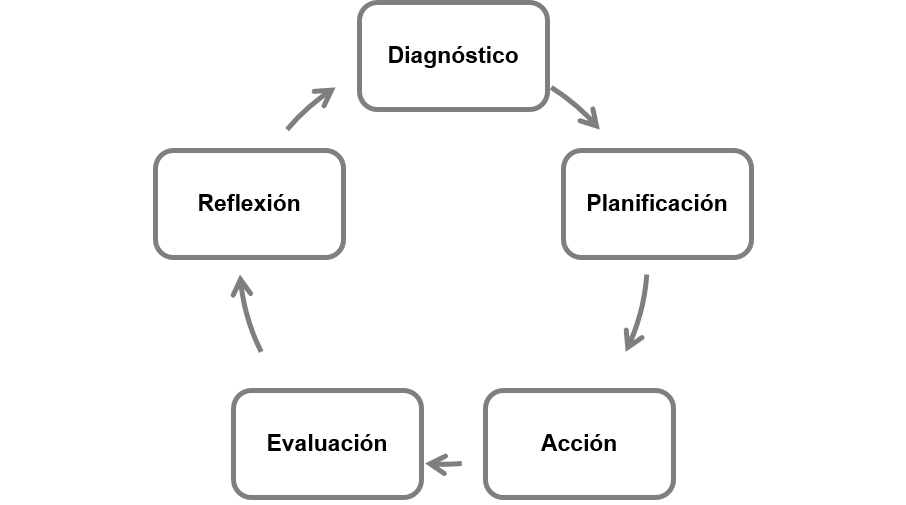
\includegraphics[scale=0.77]{img/investigacion-accion.png}
			\caption{\textbf{Figura 1.} \textit{Car\'{a}cter c\'{i}clico de Investigaci\'{o}n-Acci\'{o}n} (Fuente: Baskerville, 1999).}
	\end{figure}
	\FloatBarrier %you shall not pass table!!
	\begin{itemize}
		\item \textbf{Fase de diagn\'{o}stico:} Se realiza el proceso de identificaci\'{o}n de los problemas primarios de la investigaci\'{o}n.
		\item \textbf{Fase de planificaci\'{o}n:} Se especifican las acciones que se llevaran a cabo para solucionar los problemas primarios.
		\item \textbf{Fase de acci\'{o}n:} Se ejecutan las acciones planificadas en la fase anterior.
		\item \textbf{Fase de evaluaci\'{o}n u observaci\'{o}n:} Se efect\'{u}a una evaluaci\'{o}n de los resultados obtenidos, para observar, conocer y documentar los efectos de las acciones que fueron realizadas.
		\item \textbf{Fase de reflexi\'{o}n:} Se toman los conocimientos adquiridos en la investigaci\'{o}n-acci\'{o}n. Si las acciones ejecutadas no fueron exitosas, los conocimientos pueden proporcionar la base para el diagn\'{o}stico de un nuevo ciclo de investigaci\'{o}n-acci\'{o}n.
	\end{itemize}

En la Tabla 2 se muestran las actividades del presente proyecto, haciendo correspondencia a cada una de las fases de la Investigaci\'{o}n-Acci\'{o}n.
	\FloatBarrier %you shall not pass table!!
	\begin{table}[htb]
		\small
		\centering
		\setlength{\extrarowheight}{5pt}
		\begin{tabulary}{15cm}{|c|L|}
			\hline
			\textbf{Fase} & \textbf{Actividades}\\ \hline
			\textbf{Diagn\'{o}stico} & Identificar los problemas y limitaciones que presenta el software comercial del ``MiniScan XE Plus''.\\ \hline
			\textbf{Planificaci\'{o}n} & Seleccionar la metodolog\'{i}a de desarrollo, determinar los requisitos del software y realizar un plan de trabajo.
\\ \hline
			\textbf{Acci\'{o}n} & Desarrollar el software, tomando en cuenta los requisitos identificados previamente, los lineamientos de ingenier\'{i}a del software, est\'{a}ndares de dise\~{n}o y calidad de software.\\ \hline
			\textbf{Evaluaci\'{o}n} & Realizar las pruebas de funcionalidad del software en cuesti\'{o}n y de su interfaz gr\'{a}fica de usuario.\\ \hline
			\textbf{Reflexi\'{o}n} & Presentar los resultados y los an\'{a}lisis de las pruebas realizadas.\\ \hline
	\end{tabulary}
		\caption{\textbf{Tabla 2.} \textit{Actividades del proyecto seg\'{u}n metodolog\'{i}a Investigaci\'{o}n-Acci\'{o}n }		(Fuente: Elaboración propia).}
	\end{table}
	\FloatBarrier %you shall not pass table!!
	
	\section{Metodolog\'{i}a de Desarrollo de Software}
Para el desarrollo del software que cumpla con los objetivos planteados en esta investigaci\'{o}n y tomando en cuenta los lineamientos planteados por la ingenier\'{i}a del software, con el objetivo de obtener un software que sea fiable y que funcione eficientemente (Pressman, 2002), se ha realizado una revisi\'{o}n del enfoque que deber\'{i}a tener la metodolog\'{i}a de desarrollo a utilizar.

Seg\'{u}n Sommerville (2005, p. 361), en los a\~{n}os 80 y principios de los 90, exist\'{i}a una opini\'{o}n general de que la mejor forma de obtener un mejor software era a trav\'{e}s de una planificaci\'{o}n cuidadosa del proyecto, una garant\'{i}a de calidad formalizada, la utilizaci\'{o}n de m\'{e}todos de an\'{a}lisis y dise\~{n}o soportados por herramientas CASE, y procesos de desarrollo de software controlados y rigurosos. El software que segu\'{i}a lo mencionado previamente era desarrollado por grandes equipos que a veces trabajaban para compa\~{n}\'{i}as diferentes. A menudo estaban dispersos geogr\'{a}ficamente y trabajaban en el software durante largos periodos de tiempo.

Ahora bien, debido a que no se dispone de un equipo grande para el desarrollo del software objetivo de la presente investigaci\'{o}n, y a que no se trabajar\'{a} en \'{e}ste durante un largo periodo de tiempo, se utilizar\'{a} una metodolog\'{i}a de desarrollo de enfoque \'{a}gil. Acorde con Sommerville (2005, p. 362), los m\'{e}todos \'{a}giles dependen de un enfoque iterativo para la especificaci\'{o}n, desarrollo y entrega del software, y est\'{a}n pensados para entregar software funcional de forma r\'{a}pida a los clientes, quienes pueden entonces proponer que se incluyan en iteraciones posteriores del software nuevos requerimientos o cambios en los mismos. Si bien los m\'{e}todos \'{a}giles proponen procesos diferentes para el desarrollo y entrega incrementales de software, comparten unos principios en com\'{u}n, los cuales son ilustrados en la Tabla 3.

	\begin{table}[htb]
		\small
		\centering
		\setlength{\extrarowheight}{5pt}
		\begin{tabulary}{15cm}{|c|L|}
			\hline
			\textbf{Principio} & \textbf{Descripci\'{o}n}\\ \hline
			\textbf{Participaci\'{o}n del cliente} & Los clientes deben estar fuertemente implicados en todo el proceso de desarrollo. Su papel es proporcionar y priorizar nuevos requerimientos del software y evaluar las iteraciones del sistema.\\ \hline
			\textbf{Entrega incremental} & El software se desarrolla en incrementos, donde el cliente especifica los requerimientos a incluir en cada incremento.\\ \hline
			\textbf{Personas, no procesos} & Se deben reconocer y explotar las habilidades del equipo de desarrollo. Se les debe dejar desarrollar sus propias formas de trabajar, sin procesos formales.\\ \hline
			\textbf{Aceptar el cambio} & Se debe contar con que los requerimientos del software cambian, por lo que el software se dise\~{n}a para dar cabida a estos cambios.\\ \hline
			\textbf{Mantener la simplicidad} & Se debe centrar la simplicidad tanto en el software a desarrollar como en el proceso de desarrollo. Donde sea posible, se trabaja activamente para eliminar la complejidad del software.\\ \hline
		\end{tabulary}
		\caption{\textbf{Tabla 3.} \textit{Principios de los m\'{e}todos \'{a}giles} (Fuente: Sommerville, 2005).}
	\end{table}

		\subsection{Metodolog\'{i}a SCRUM}
De acuerdo con Schwaber y Sutherland (2013, p. 4), esta metodolog\'{i}a es un marco de trabajo por el cual las personas pueden acometer problemas complejos adaptativos, y a la vez entregar productos del m\'{a}ximo valor posible, productiva y creativamente. SCRUM no es un proceso o una t\'{e}cnica para construir productos; en lugar de eso, es un marco de trabajo dentro del cual se pueden emplear varias t\'{e}cnicas y procesos. 
			
		\newpage			
			
El marco de trabajo SCRUM consiste en los equipos SCRUM, roles, eventos, artefactos y reglas asociadas. Cada componente dentro del marco de trabajo sirve a un prop\'{o}sito espec\'{i}fico y es esencial para el \'{e}xito de SCRUM y para su uso (Schwaber y Sutherland, 2013, p. 4).

SCRUM se basa en la teor\'{i}a de control de procesos emp\'{i}rica. El empirismo asegura 	que el conocimiento procede de la experiencia y de tomar decisiones bas\'{a}ndose en lo que se conoce. Esta metodolog\'{i}a emplea un enfoque iterativo e incremental para optimizar la predictibilidad y el control de riesgo. La implementaci\'{o}n de este control de procesos est\'{a} soportada por tres pilares, los cuales se muestran en la Tabla 4.
			
			\begin{table}[htb]
				\small
				\centering
				\setlength{\extrarowheight}{5pt}
				\begin{tabulary}{15cm}{|c|L|}
					\hline
					\textbf{Pilar} & \textbf{Descripci\'{o}n}\\ \hline
					\textbf{Transparencia} & Los aspectos significativos del proceso deben ser visibles para aquellos que son responsables del resultado.\\ \hline
					\textbf{Inspecci\'{o}n} & Los usuarios SCRUM deben inspeccionar frecuentemente los artefactos de SCRUM y el proceso hacia un objetivo, para detectar variaciones.\\ \hline
					\textbf{Adaptaci\'{o}n} & Si un inspector determina que uno o m\'{a}s aspectos de un proceso se desv\'{i}an de l\'{i}mites aceptables, y que el producto resultante no ser\'{a} aceptable, el proceso o el material que est\'{a} siendo procesado debe ser ajustado.\\ \hline
			\end{tabulary}
			\caption{\textbf{Tabla 4.} \textit{Pilares del control de procesos de SCRUM} (Fuente: Elaboraci\'{o}n propia).}
			\end{table}
			\newpage
			
Adicionalmente a la utilizaci\'{o}n de la metodolog\'{i}a SCRUM, se incluyeron algunos
artefactos de la metodolog\'{i}a RUP (Rational Unified Process), para as\'{i} generar suficiente documentaci\'{o}n durante el dise\~{n}o y el desarrollo del nuevo software. La configuraci\'{o}n
 de la metodolog\'{i}a SCRUM utlizada en conjunto con los artefactos elegidos de la
 metodolog\'{i}a RUP, es la ilustrada en la Tabla 5.

			\begin{table}[htb]
				\small
				\centering
				\setlength{\extrarowheight}{5pt}
			\begin{tabulary}{15cm}{|L|L|}
				\hline
				\textbf{Artefactos SCRUM}\\ \hline
				\textbf{Backlog de producto: }Lista din\'{a}mica de las cosas que se deben hacer, sin especificar c\'{o}mo se deben hacer.\\ \hline
				\textbf{Backlog de sprint: }Recopilaci\'{o}n sint\'{e}tica de los \'{i}tems del backlog del producto, en donde se quiebran los \'{i}tems en tareas peque\~{n}as que no demanden una labor superior a una jornada de trabajo.\\ \hline
				\textbf{Incremento de funcionalidad: }Es lo que el equipo SCRUM entrega la final de cada sprint. El mismo debe asemejarse a un software funcionando, permitiendo implementarse operativamente sin restricciones en un ambiente productivo.\\ \hline
				\textbf{Artefactos RUP}\\ \hline
				\textbf{Documento de Visi\'{o}n: }Documento que define el alcance de alto nivel y prop\'{o}sito del producto.\\
\hline
				\textbf{Glosario: }Documento que define la terminolog\'{i}a empleada en los artefactos.\\ \hline
				\textbf{Configuraci\'{o}n de documentos de requerimientos:} Solamente requerimientos no funcionales.\\ \hline
		\textbf{Configuraci\'{o}n de documentos de arquitectura: } Solamente diagrama de Casos de Uso.\\ \hline
			\end{tabulary}
	\caption{\textbf{Tabla 5.} \textit{Configuraci\'{o}n de los artefactos a utilizar de SCRUM y RUP} (Fuente: Elaboraci\'{o}n propia).}
			\end{table}